\section{Machine Learning Models}
\label{sec:ML_Models}
\subsection{Introduction}
In this section, we present and discuss the machine learning models implemented in this project, focusing on their structure, functionality, and contributions to the problem at hand. These models fall within the supervised learning paradigm and are specifically designed to address the challenges of scene image classification.

We begin with an in-depth exploration of several neural network architectures, including Feedforward Neural Networks (FNNs), Convolutional Neural Networks (CNNs), and DenseNet. Each model leverages unique mechanisms to process and learn from the data, enabling accurate classification of images into multiple categories. Furthermore, we describe the hyperparameter tuning strategies employed to optimize these models for enhanced performance, as well as the data augmentation techniques used to enrich the training dataset and improve model generalization.

Finally, we outline the evaluation metrics and hyperparameters used to assess the models’ effectiveness. These metrics provide a comprehensive understanding of the models’ predictive accuracy, robustness, and suitability for the classification task. 


\subsection{Feedforward Neural Networks}
A Feedforward Neural Network (FNN) is one of the simplest forms of artificial neural networks. It is designed to approximate functions by mapping input data to output labels through a series of hidden layers. Unlike more complex architectures, FNNs process information in one direction—from the input layer, through the hidden layers, to the output layer—without forming cycles or loops.


\begin{figure}[h!]
    \centering
    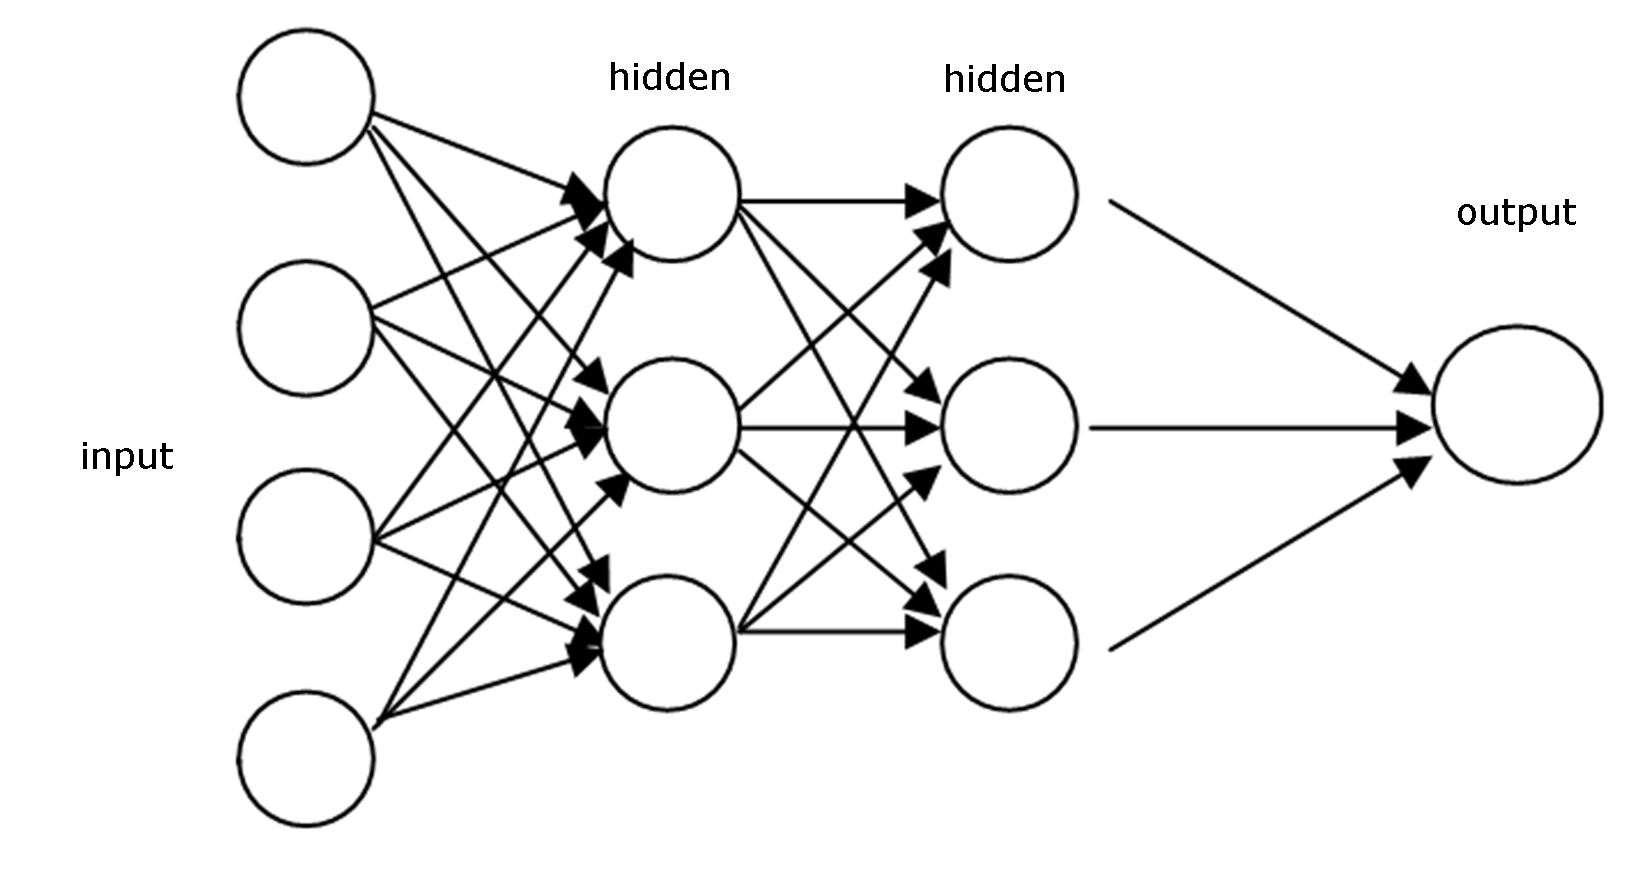
\includegraphics[width=0.8\linewidth]{images/feedforward_structure.png}
    \caption{Structure of a Feedforward Neural Network}
    \label{fig:feedforward_structure}
\end{figure}

Each neuron in a Feedforward Neural Network is a computational unit that applies a weighted sum of its inputs, adds a bias, and passes the result through an activation function. Mathematically, this process can be expressed as:
\[
y = f\left(\sum_{i=1}^{n} w_i x_i + b\right)
\]
where:

- \(y\) is the neuron's output,

- \(x_i\) are the inputs,

- \(w_i\) are the weights associated with the inputs,

- \(b\) is the bias term,

- \(f\) is the activation function (e.g., Sigmoid, ReLU, or Tanh).


A Feedforward Neural Network consists of three main types of layers:

1. Input Layer: This layer receives the input data and serves as the network's entry point. Each node in this layer represents a feature of the input data.

2. Hidden Layers: These layers perform the bulk of the computation in the network. Each hidden layer applies a transformation to the data using weights, biases, and activation functions. The number of hidden layers and their respective sizes define the network's capacity to model complex functions.

3. Output Layer: This layer produces the network's predictions. For classification tasks, the output layer typically applies a Softmax activation function to generate probabilities for each class.

\begin{figure}[h!]
    \centering
    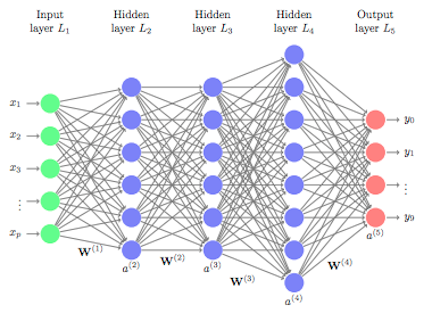
\includegraphics[width=1\linewidth]{images/feedforward_workflow.png}
    \caption{Workflow of a Feedforward Neural Network}
    \label{fig:feedforward_workflow}
\end{figure}

The workflow of a Feedforward Neural Network can be summarized as follows. First, during forward propagation, the input data passes through the network layer by layer. Each layer performs a linear transformation on the inputs, followed by the application of a non-linear activation function. The final layer then generates predictions, which can be probabilities in the case of classification tasks or continuous values for regression tasks.

Next, the loss calculation step measures the difference between the predicted outputs and the true labels using a loss function. 

Following this, backpropagation is performed to update the network's parameters. In this step, the gradient of the loss function with respect to each weight and bias is computed using the chain rule. These gradients are propagated backward through the network, allowing the parameters to be adjusted to minimize the loss.

Finally, during optimization, an algorithm such as Gradient Descent or Adam uses the calculated gradients to iteratively update the weights and biases, thereby improving the network's performance and enabling it to learn from the data.

Feedforward Neural Networks are foundational in deep learning, commonly used for structured data and simple tasks. While not ideal for large-scale image classification due to their lack of specialized operations, they are included here to observe their behavior and compare with more advanced architectures.

\subsection{Convolutional Neural Networks}
%To understand the structure and function of a Convolutional Neural Network (CNN), it is essential first to grasp the basic concept of a Neural Network (NN). A Neural Network consists of an input layer, one or more hidden layers, and an output layer. The input layer receives training data, while the hidden layers perform the computational processes that lead to the output layer, which produces the results. The next figure illustrates the structure of a Neural Network, showcasing the connections between layers, where each connection is associated with a weight. These weights represent the "cost" or influence of one neuron on another.

%\begin{figure}[h!]
%    \centering
%    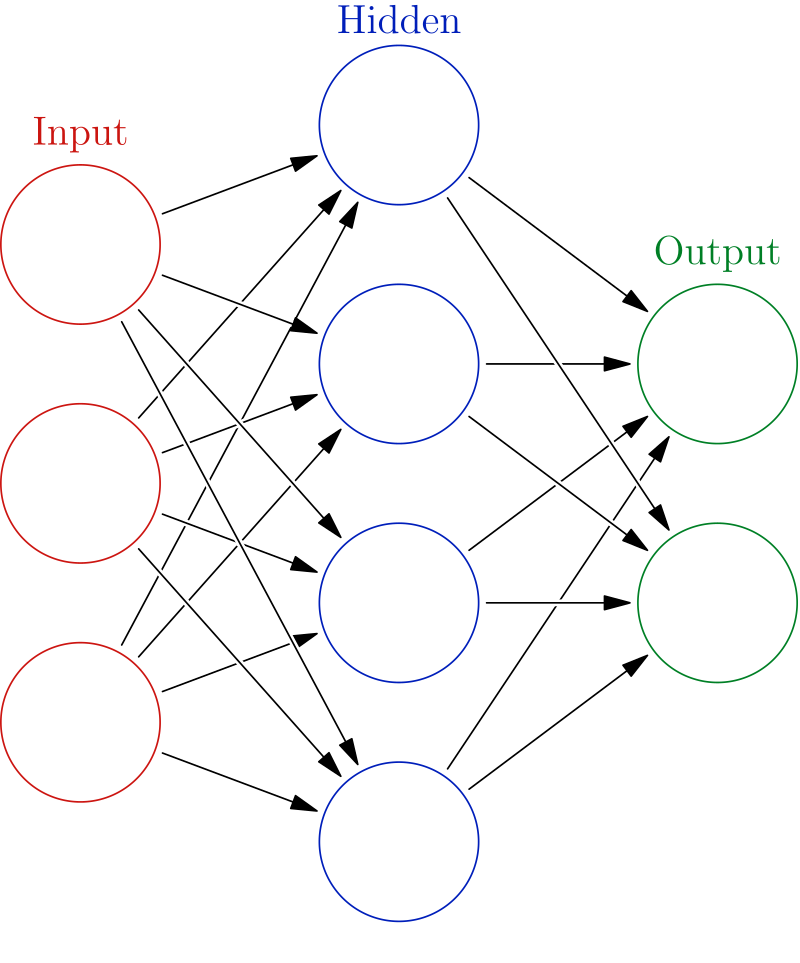
\includegraphics[width=0.75\linewidth]{images/NN_struture.png}
%    \caption{NN Struture}
%    \label{fig:enter-label}
%\end{figure}

%However, traditional Neural Networks face significant challenges when 
Traditional Neural Networks such as FNNs face significant challenges when applied to image data. For instance, an image of size 100×100×3 (height, width, and color channels) contains 30,000 features per image. If every feature is connected to all neurons in the next layer, the model becomes computationally prohibitive and prone to overfitting due to insufficient training data. And to worsen this, they lack specific mechanisms to capture the spatial relationships between image pixels. These limitations make standard Neural Networks unsuitable for complex image classification tasks.

CNNs overcome these limitations by employing convolution, a specialized operation designed to efficiently process image data. Convolution is mathematically defined as the sum of element-wise products between two matrices—a filter and a segment of the input image. This process is illustrated in Figure \ref{fig:conv_process}.

\begin{figure}[h!]
    \centering
    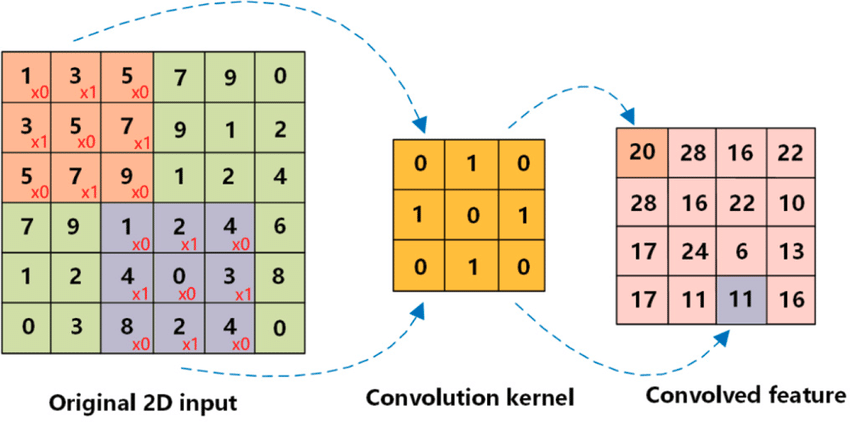
\includegraphics[width=1\linewidth]{images/convolution_process.png}
    \caption{Convolution Process}
    \label{fig:conv_process}
\end{figure}

Filters are fundamental to CNNs, acting as templates for detecting specific features such as edges, textures, or patterns within the input image. As a filter is convolved across the image, it generates a feature map that highlights regions closely matching the filter's pattern. The dimensions of the feature map are determined by the formula:
\[
(n - f + 1) \times (n - f + 1)
\]
where \(n \space = \space  n \times n \) is the input image size, and \( f \space = \space f \times f \) is the filter size.

One challenge of convolution is that it reduces the image size with each operation, potentially discarding valuable edge and corner information. To mitigate this, padding is used. Padding adds extra layers of pixels around the image’s borders, preserving edge and corner details during convolution. 
\begin{figure}[h!]
    \centering
    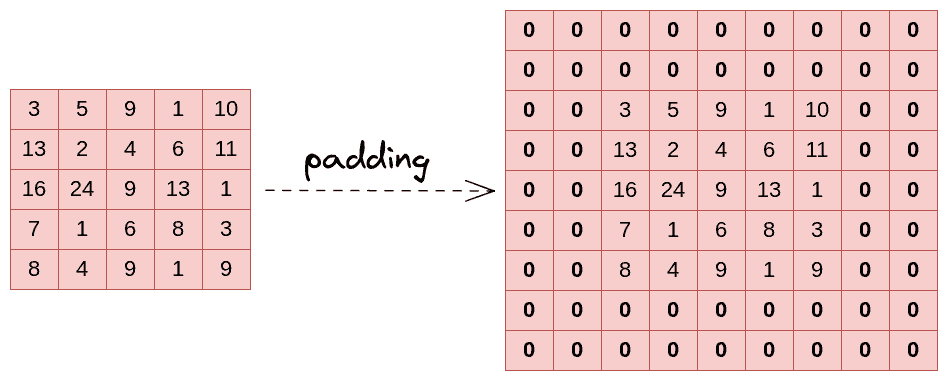
\includegraphics[width=1\linewidth]{images/padding.png}
    \caption{Padding}
    \label{fig:enter-label}
\end{figure}


Another critical CNN component is the pooling layer, which summarizes feature maps by reducing their spatial dimensions. This compression minimizes the number of parameters, making the model more robust and less sensitive to the exact positions of features. In this study, max pooling is employed, selecting the maximum value from each sub-matrix of the feature map. This technique ensures that the most prominent feature in each region is retained, as shown in the next figure.

\begin{figure}[h!]
    \centering
    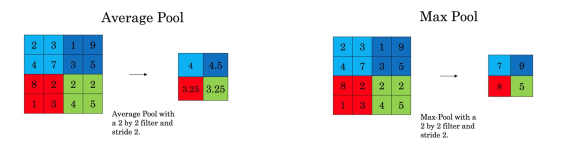
\includegraphics[width=1\linewidth]{images/Pooling.png}
    \caption{Pooling layer}
    \label{fig:enter-label}
\end{figure}


A CNN performs multiple cycles of convolution and pooling to extract hierarchical features from the input image. After these layers, the resulting feature maps are flattened into a one-dimensional vector. This flattened vector serves as the input to a fully connected layer, where the process continues like a standard Neural Network, leading to the final classification output.

\begin{figure}[h!]
    \centering
    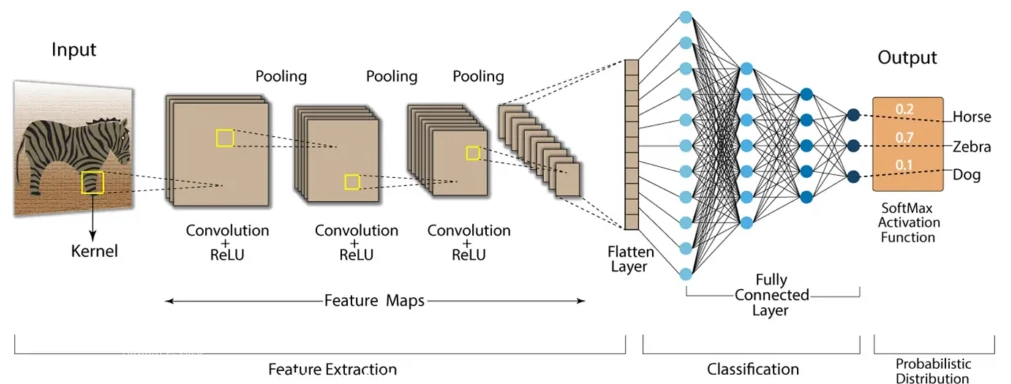
\includegraphics[width=1\linewidth]{images/CNN_example.png}
    \caption{CNN Structure}
    \label{fig:enter-label}
\end{figure}

By combining convolution, pooling, and fully connected layers, CNNs effectively reduce computational requirements and improve accuracy for tasks like image classification, making them an ideal choice for this study.



\subsection{DenseNet}
DenseNet, short for Densely Connected Convolutional Network, is an advanced architecture for deep learning that aims to address some of the limitations of traditional CNNs. Introduced to enhance gradient flow and improve parameter efficiency, DenseNet achieves this by ensuring direct connections between each layer and all subsequent layers, as illustrated in the figure below.

\begin{figure}[h!]
    \centering
    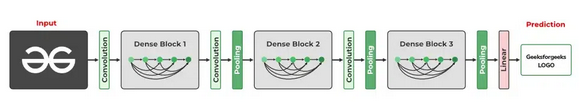
\includegraphics[width=1\linewidth]{images/dense_net_arquitetura.png}
    \caption{Architecture of DenseNet}
    \label{fig:enter-label}
\end{figure}

In DenseNet, every layer receives the feature maps of all preceding layers as input and passes its feature maps to all subsequent layers. This approach contrasts with traditional CNNs, where layers are connected sequentially. DenseNet’s dense connectivity can be mathematically represented as:
\[
x_l = H_l([x_0, x_1, ..., x_{l-1}])
\]

- \(x_l\) represents the output of the \(l\)-th layer.

- \(H_l\) denotes the composite function (e.g., Batch Normalization, ReLU, and Convolution).

- \([x_0, x_1, ..., x_{l-1}]\) represents the concatenation of the feature maps from all preceding layers.

This dense connectivity pattern significantly reduces redundancy, promotes feature reuse, and alleviates the vanishing gradient problem.



DenseNet introduces transition layers to manage the model's size and reduce the spatial dimensions of feature maps. These layers consist of Batch Normalization, a \(1 \times 1\) convolutional operation, and \(2 \times 2\) average pooling. The transition layers ensure that the network remains compact and computationally efficient while preserving important features.

\begin{figure}[h!]
    \centering
    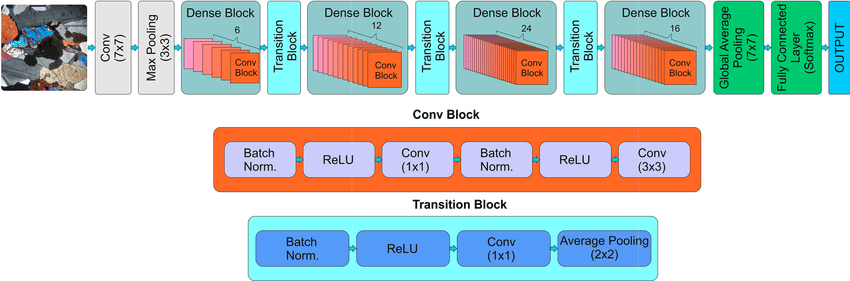
\includegraphics[width=1\linewidth]{images/DenseNet_transition.png}
    \caption{DenseNet Transition Layer}
    \label{fig:densenet_transition}
\end{figure}

Dense blocks are the core components of DenseNet, where the dense connectivity occurs. Within a dense block, each layer has access to the feature maps of all previous layers, promoting efficient feature propagation and reuse. Let \(k\) denote the growth rate, which determines the number of feature maps each layer contributes. The feature map count in a dense block grows linearly with the number of layers.

The output of a dense block with \(L\) layers can be expressed as:
\[
\text{Output feature maps} = k \cdot L
\]
where \(k\) is a hyperparameter chosen based on the model's complexity requirements.


\begin{figure}[h!]
    \centering
    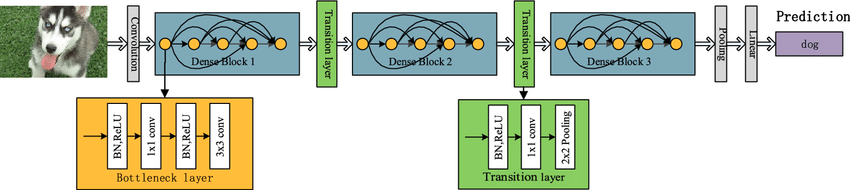
\includegraphics[width=1\linewidth]{images/DenseNet_workflow.png}
    \caption{DenseNet Example}
    \label{fig:densenet_workflow}
\end{figure}

The workflow of DenseNet combines dense blocks and transition layers to achieve an efficient and compact model structure. 

1. Input Layer: The input image is first processed by an initial convolutional layer to extract basic features.

2. Dense Block: Each dense block performs iterative feature extraction, where each layer has direct access to all previous layers' feature maps. This promotes feature reuse and minimizes redundancy.

3. Transition Layer: Between dense blocks, transition layers reduce the spatial dimensions and feature map count, ensuring computational efficiency and controlling model size.

4. Final Classification: After passing through a series of dense blocks and transition layers, the feature maps are global average pooled, flattened, and fed into a fully connected layer for the final classification output.

This structured workflow ensures that DenseNet achieves superior gradient flow, efficient parameter use, and excellent feature extraction capabilities, making it a powerful architecture for tasks like image classification, making them an ideal choice for this study.


\subsection{Data Augmentation and Hyperparameter Tuning}

To enhance the performance and generalization of the machine learning models, this study employs two critical techniques: data augmentation and hyperparameter tuning.

\subsubsection{Data Augmentation}
Data augmentation is applied to artificially increase the diversity and size of the training dataset, mitigating overfitting and improving the models' ability to generalize to unseen data. This is achieved by applying transformations such as random rotations, flips, zooming, cropping, and changes in brightness or contrast to the input images. These transformations introduce variability while preserving the semantic meaning of the data, ensuring that the models learn robust features rather than overfitting to specific patterns in the original dataset.

\begin{figure}[h!]
    \centering
    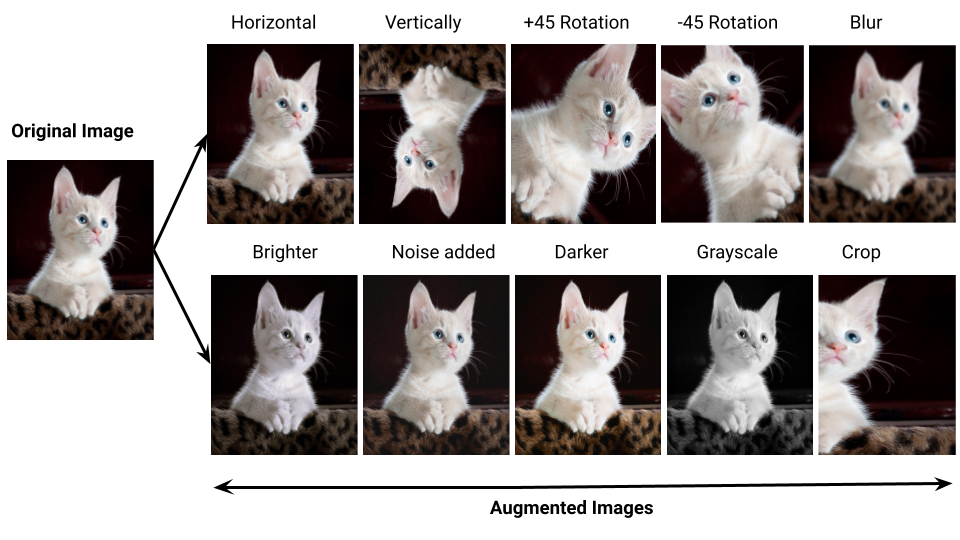
\includegraphics[width=0.9\linewidth]{images/data_augmentation.png}
    \caption{Data Augmentation examples}
    \label{fig:enter-label}
\end{figure}

\subsubsection{Hyperparameter Tuning}
Hyperparameter tuning involves systematically optimizing the key parameters that govern the training process and architecture of the models. Examples of hyperparameters include the learning rate, batch size, number of layers, number of neurons per layer, and dropout rates. This process is conducted using techniques like grid search or random search to identify the optimal combination of hyperparameters that maximize the models' performance on the validation dataset. Tuning ensures that the models achieve a balance between underfitting and overfitting, leading to better overall accuracy and generalization.

\hfill


By integrating data augmentation and hyperparameter tuning into the training workflow, the implemented models are better equipped to handle the challenges of scene image classification, yielding improved accuracy and robustness in their predictions. At the end of the study, the results will be compared across various configurations, including baseline models without augmentation or tuning, models with data augmentation, and models with optimized hyperparameters, to evaluate the impact of these techniques on performance.



\subsection{Model Evaluation: Confusion Matrix and Classification Metrics}
The evaluation of the models will be carried out using the confusion matrix, which provides a detailed view of the model’s correct and incorrect predictions for each class (e.g., road, forest, etc.). In addition, classification metrics including \textit{accuracy}, \textit{precision}, \textit{recall}, and \textit{F1-score} will be calculated. These metrics are essential for assessing the effectiveness of the model in differentiating between various scene types.

\subsubsection{Confusion Matrix}
A confusion matrix is a table that
indicates the mistakes and successes of your model, comparing to the expected result, the layout of a confusion matrix in present on the next figure. We will utilize to compute the confusion matrix, which is the sklearn function of confusion matrix.

\begin{figure}[h!]
    \centering
    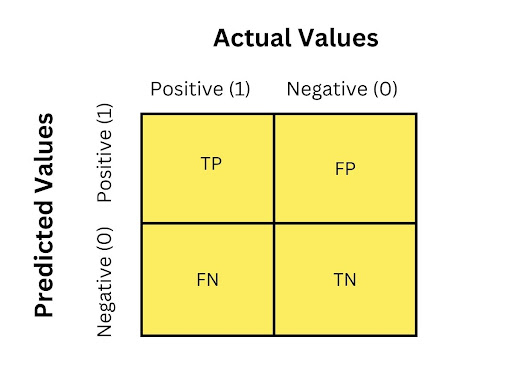
\includegraphics[width=0.75\linewidth]{images/confusion_matrix.png}
    \caption{Confusion Matrix}
    \label{fig:enter-label}
\end{figure}


\subsubsection{Precision}
Precision score, a vital metric in evaluating classification models, measures the ratio of true positive predictions to the total number of positive predictions made by the model. It provides insight into the model’s ability to correctly identify relevant instances from all instances predicted as positive.
The precision score is calculated as:
\[Precision=\frac{True Positives (TP)}{True Positives (TP)+False Positives (FP)}\]

\subsubsection{Recall (Sensitivity)}
Recall score, also known as sensitivity or true positive rate, gauges the model’s ability to correctly identify all relevant instances from the total number of actual positive instances in the dataset.
Its formula is the following:
\[Recall=\frac{True Positives (TP)}{True Positives (TP)+False Negatives (FN)}\]

\subsubsection{F1-Score}
The F1 score, a harmonic mean of precision
and recall, provides a balanced assessment of a model’s
performance. It combines both precision and recall into a
single metric, making it useful for evaluating models with imbalanced class distributions.
\[F1Score=2 \times \frac{Precision*Recall}{Precision+Recall}\]

\subsubsection{Accuracy}
Accuracy is the proportion of correct predictions (both true positives and true negatives) to the total number of predictions made. It represents the overall correctness of the model's predictions. It is especially usefull when the dataset is balanced.
\[Accuracy= \frac{True Positives (TP)\times True Negatives (TN)}{Total Predictions}\]


\subsubsection{Training Loss}
Training loss quantifies how well the model fits the training data by calculating the difference between predicted and actual values. It is computed using a loss function such as cross-entropy for classification or mean squared error for regression. A lower loss means better model predictions. The goal during training is to minimize loss, but low training loss doesn’t always imply good generalization—overfitting can occur if the model is too closely fit to the training data.

\subsubsection{ROC curve graph}
The ROC (Receiver Operating Characteristic) curve is a graphical representation used to evaluate the performance of binary classifiers. It shows the trade-off between the True Positive Rate (TPR) and False Positive Rate (FPR) as the classification threshold varies. TPR is also known as sensitivity, and FPR is 1 - specificity.

% True Positive Rate (TPR)
\[
\text{TPR} = \frac{\text{True Positives (TP)}}{\text{True Positives (TP)} + \text{False Negatives (FN)}}
\]

% False Positive Rate (FPR)
\[
\text{FPR} = \frac{\text{False Positives (FP)}}{\text{False Positives (FP)} + \text{True Negatives (TN)}}
\]

The curve is plotted with the False Positive Rate (FPR) on the x-axis and the True Positive Rate (TPR) on the y-axis. Each point on the curve corresponds to a different threshold for classifying positive and negative outcomes.

\begin{figure}[h!]
    \centering
    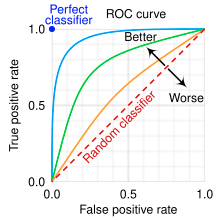
\includegraphics[width=0.75\linewidth]{images/roc.png}
    \caption{ROC Example}
    \label{fig:enter-label}
\end{figure}

The Area Under the Curve (AUC) summarizes the model's overall performance. A perfect classifier has an AUC of 1, while a random classifier has an AUC of 0.5. The ROC curve helps in selecting an optimal threshold for balancing sensitivity and specificity according to the specific requirements of the problem.

